% arXiv builds through DVI unless told otherwise, and the DVI route cannot embed
% PNG. This paper loads orcid.png and figures/help.png, so pdfLaTeX is required.
% arXiv reads this declaration only within the first five lines of the main file.
\pdfoutput=1

\documentclass{article}

\usepackage{arxiv}

\usepackage[utf8]{inputenc}
\usepackage[T1]{fontenc}
\usepackage{hyperref}
\usepackage{url}
\usepackage{booktabs}
\usepackage{amsfonts}
\usepackage{amsmath}
\usepackage{amssymb}
\usepackage{amsthm}
\usepackage{microtype}
\usepackage{graphicx}
\usepackage{natbib}
\usepackage{doi}
\usepackage{xcolor}
\usepackage{tikz}
\usetikzlibrary{arrows.meta, positioning, calc}

% -----------------------------------------------------------------------------
% The five lifecycle colours, shared by every figure here and by the poster, the
% slides and the demonstration. Fills take the !12 tint, strokes the full colour.
% -----------------------------------------------------------------------------
\definecolor{acquire} {HTML}{4A7FD4}
\definecolor{store}   {HTML}{2A9D8F}
\definecolor{retrieve}{HTML}{E08A2E}
\definecolor{update}  {HTML}{D05353}
\definecolor{forget}  {HTML}{8F5FB8}
\definecolor{muted}   {HTML}{4A4A55}
\usepackage{enumitem}
\usepackage{caption}
\usepackage{algorithm}
\usepackage{algpseudocode}

\newtheorem{proposition}{Proposition}
\newtheorem{assumption}{Assumption}

% Custom marks for comparison tables
\newcommand{\fullmark}{\checkmark}
\newcommand{\halfmark}{$\sim$}

\hypersetup{
  colorlinks=true,
  linkcolor=blue!70!black,
  citecolor=green!50!black,
  urlcolor=blue!60!black,
  pdftitle={The Knowledge Lifecycle of Large Language Models},
  pdfsubject={cs.CL},
  pdfauthor={Amey Thakur, Sarvesh Talele},
  pdfkeywords={Large Language Models, Knowledge Lifecycle, RAG, Knowledge Editing, Continual Learning, Machine Unlearning},
}

\title{The Knowledge Lifecycle of Large Language Models}

\author{
	\href{https://orcid.org/0000-0001-5644-1575}{
\includegraphics[scale=0.06]{orcid.png}\hspace{1mm}Amey Thakur} \\
	Independent Researcher \\
	Toronto, Canada \\
	\texttt{ameythakur20@gmail.com} \\
	\And
	\href{https://orcid.org/0009-0002-0818-461X}{
\includegraphics[scale=0.06]{orcid.png}\hspace{1mm}Sarvesh Talele} \\
	Independent Researcher \\
	Mumbai, India \\
	\texttt{talelesarvesh@gmail.com} \\
}

\renewcommand{\undertitle}{}
\renewcommand{\headeright}{}
\renewcommand{\shorttitle}{The Knowledge Lifecycle of LLMs}

\begin{document}
\maketitle

\begin{abstract}
Reasoning models and inference-time scaling have changed how large language models (LLMs) handle knowledge: earlier systems used static pipelines of retrieval-augmented generation (RAG), knowledge editing, and continual learning, while modern systems resolve conflicts during test-time compute. No unified formalism describes how knowledge persists, evolves, and is computed over across a model's lifespan. We introduce the \textbf{Knowledge Lifecycle}, which organizes LLM knowledge management into five stages: \textit{Acquisition}, \textit{Storage}, \textit{Retrieval}, \textit{Update}, and \textit{Forgetting}. We formalize the five stages and their cross-stage failure modes, showing that subfields addressing each stage in isolation leave the boundaries between them unstudied. We propose the \textbf{Provenance Vector} ($p$), which stores temporal and source metadata alongside parametric memories and gates stale activations at inference, and \textbf{Lifecycle Desynchronization} ($\mathcal{D}_{sync}$), a Kullback-Leibler metric for the failure that occurs when parametric weights and retrieved context conflict. In a reproducible probe of a documented drug withdrawal, GPT-2 gives the correct continuation probability $5.9 \times 10^{-6}$ with the withdrawal notice in context ($\mathcal{D}_{sync} = 12.05$ nats), while that context shifts its output distribution by $0.033$ nats. Across six open models from 124M to 1.5B parameters and three documented fact changes the conflict does not resolve with scale: no model answers the withdrawal probe correctly, and within one family the measurement is not monotone in size. Other conflicts in the same set do resolve, so the metric tracks the conflict rather than question difficulty. Wording matters too: across three phrasings per probe the Vioxx measurement has a median standard deviation of 5.14 nats and the phrasing reported here is the hardest for every model tested, so $\mathcal{D}_{sync}$ describes a conflict together with the query that probes it.
\end{abstract}

\section*{List of Abbreviations}
\begin{description}[style=multiline, leftmargin=3cm, font=\bfseries]
  \item[LLM] Large Language Model
  \item[RAG] Retrieval-Augmented Generation
  \item[KL] Kullback-Leibler (divergence)
  \item[RLHF] Reinforcement Learning from Human Feedback
  \item[RepE] Representation Engineering
  \item[FFN] Feed-Forward Network
  \item[VLM] Vision-Language Model
  \item[FDA] Food and Drug Administration
  \item[MIPS] Maximum Inner Product Search
  \item[CE] Cross-Entropy
  \item[MSE] Mean Squared Error
  \item[DPR] Dense Passage Retrieval
  \item[ROME] Rank-One Model Editing
  \item[MEMIT] Mass-Editing Memory in Transformers
  \item[LoRA] Low-Rank Adaptation
  \item[EWC] Elastic Weight Consolidation
\end{description}

% ============================================================
\section{Introduction}
\label{sec:introduction}
% ============================================================

Large language models serve as the backbone of systems that answer medical questions, draft legal briefs, write production code, and tutor students in mathematics~\citep{brown2020language, achiam2023gpt4, team2023gemini}. With the advent of inference-time scaling and reasoning models such as OpenAI o1 and DeepSeek-R1~\citep{openai2024o1, guo2025deepseekr1}, these systems no longer simply retrieve and generate; they execute extended test-time compute to search, reflect, and self-correct. That reasoning is bound by a bottleneck beneath it: the model's relationship with the facts it reasons over. A medical reasoning agent that computes over a retracted drug interaction, or a coding agent that builds logic around a deprecated API, represents a failure of knowledge management rather than a failure of reasoning capacity.

Current responses to these challenges are fragmented. General surveys on LLMs~\citep{zhao2023surveyllm, wang2024agents} touch on knowledge tangentially, while specific subfields operate in isolation. At least five separate subfields now address different pieces of the knowledge problem:

\begin{enumerate}[leftmargin=*]
  \item \textbf{Retrieval-Augmented Generation (RAG)} focuses on how to fetch relevant documents and feed them to the model at inference time~\citep{lewis2020rag, guu2020realm, gao2023ragsurvey}.
  \item \textbf{Knowledge Editing} asks whether individual facts inside a model's weights can be surgically modified without retraining~\citep{meng2022rome, meng2023memit, yao2023editingsurvey}.
  \item \textbf{Continual Learning} tackles how a model can absorb new information over time without destroying what it already knows~\citep{kirkpatrick2017ewc, ke2023continual, wu2024continual}.
  \item \textbf{Context Engineering} studies how to arrange, compress, and prioritize information within a finite context window~\citep{liu2024lost}.
  \item \textbf{Agent Memory} builds persistent storage that lets LLM-based agents remember and reuse past experience~\citep{park2023generative, packer2023memgpt, hu2025agentmemory}.
\end{enumerate}

Each subfield has its own dedicated surveys~\citep{gao2023ragsurvey, mialon2023augmented, hu2025agentmemory, wu2025humanmemory}. They rarely integrate their methodologies. Optimizing a RAG retriever seldom includes an evaluation of what happens when retrieved facts contradict the model's parametric memory. A team building a knowledge editor rarely checks whether their edits survive continual fine-tuning. These isolated evaluations obscure cross-stage system failures.

This paper proposes an integrated approach. Rather than treating these problems in isolation, we formalize them as stages of a single unified architecture: the \textbf{Knowledge Lifecycle} of large language models. The lifecycle defines five structural stages: how knowledge is \textit{acquired}, \textit{stored}, and \textit{retrieved} (\S\ref{sec:legacy_pipeline}), how it is \textit{updated} as the world changes (\S\ref{sec:update}), and how it is \textit{forgotten}, whether deliberately or by accident (\S\ref{sec:forgetting}).

\paragraph{Contributions.} We make three contributions:

\begin{enumerate}[leftmargin=*]
  \item \textbf{A lifecycle framework} that unifies existing research across five structural stages (\S\ref{sec:framework}--\S\ref{sec:analysis}). We formalize the operational mechanics of each stage and map twenty representative works onto the stages they address, showing that the boundaries between stages are where the least-studied and most damaging failures occur.

  \item \textbf{The Provenance Vector ($p$)} (\S\ref{sec:contributions}), an architectural proposal that stores temporal and source metadata alongside each parametric memory. A gating function reads this metadata during inference and suppresses stale activations, allowing retrieved context to dominate without destructive weight edits. We give the forward pass as an explicit algorithm, derive the parameter overhead, and prove an idealized consistency result with clearly stated assumptions.

  \item \textbf{Lifecycle Desynchronization ($\mathcal{D}_{sync}$)} (\S\ref{sec:contributions}), an evaluation metric that measures the failure occurring when model weights are out of sync with external retrieval indices. We define the metric, give its measurement protocol as an algorithm, and report a reproducible probe on GPT-2 in which the correct continuation receives probability $5.9 \times 10^{-6}$ despite the corrective document being present in context.
\end{enumerate}

To our knowledge, no prior work has formalized the knowledge management problem across all five lifecycle stages.

\paragraph{Reproducibility and artifacts.} Every measurement reported in this paper is produced by a single deterministic script: no sampling is used anywhere, so the values reproduce exactly on any machine. The script, the manuscript source, and the cross-model measurement notebook are released as an open repository~\citep{thakur2026code}. We additionally release an interactive demonstration~\citep{thakur2026demo}, which executes GPT-2 entirely in the reader's browser through ONNX, requires no installation or credentials, and reproduces the measurement of \S\ref{sec:case_study} exactly. It accepts arbitrary conflict pairs, so a reader may test the metric against a fact change of their own choosing before reading further.

% ============================================================
\section{Background and Scope}
\label{sec:background}
% ============================================================

\subsection{What Counts as ``Knowledge'' in an LLM?}

We use ``knowledge'' broadly. Within the Knowledge Lifecycle framework, knowledge is any information, whether factual, procedural, or experiential, that shapes a model's outputs. Four varieties matter here:

\begin{itemize}[leftmargin=*]
  \item \textbf{Factual knowledge.} Concrete facts about the world (``The boiling point of water at sea level is 100\textdegree C''), acquired mainly during pre-training~\citep{petroni2019lama}.
  \item \textbf{Procedural knowledge.} How to carry out tasks: following multi-step instructions, writing code in a particular style, or reasoning through a chain of logic. This is typically instilled through instruction tuning and Reinforcement Learning from Human Feedback (RLHF)~\citep{ouyang2022instructgpt, wei2022flan}.
  \item \textbf{Experiential knowledge.} Records of past interactions, user preferences, and task outcomes kept by agent memory systems~\citep{park2023generative, packer2023memgpt}.
  \item \textbf{Contextual knowledge.} Information provided at inference time via the prompt or fetched from an external source~\citep{lewis2020rag}.
\end{itemize}

The same fact can exist in several forms at once. ``The CEO of OpenAI is Sam Altman'' might live in the model's weights (parametric), in a vector database (non-parametric), and in the current prompt (contextual). Each copy follows a different lifecycle path, with different update and deletion properties.

\subsection{Relationship to Existing Literature}

Table~\ref{tab:survey_comparison} shows where prior literature sits. Each subfield covers one or two lifecycle stages in depth; none attempts the full picture.

\begin{table}[t]
\centering
\caption{Coverage of lifecycle stages in prior literature. \fullmark\ = primary focus; \halfmark\ = partial; -- = absent.}
\label{tab:survey_comparison}
\small
\begin{tabular}{@{}lccccc@{}}
\toprule
\textbf{Work} & \textbf{Acquire} & \textbf{Store} & \textbf{Retrieve} & \textbf{Update} & \textbf{Forget} \\
\midrule
Gao et al.\ (2023), on RAG & -- & \halfmark & \fullmark & -- & -- \\
Mialon et al.\ (2023), Augmented LMs & \halfmark & -- & \fullmark & -- & -- \\
Yao et al.\ (2023), Knowledge Editing & -- & \halfmark & -- & \fullmark & -- \\
Wu et al.\ (2024), Continual Learning & \halfmark & -- & -- & \fullmark & \halfmark \\
Hu et al.\ (2025), Agent Memory & -- & \fullmark & \fullmark & \halfmark & \halfmark \\
Wu et al.\ (2025), Human$\to$AI Memory & \halfmark & \fullmark & \halfmark & \halfmark & -- \\
\midrule
\textbf{Our framework} & \fullmark & \fullmark & \fullmark & \fullmark & \fullmark \\
\bottomrule
\end{tabular}
\vspace{-1em}
\end{table}

Three works require explicit differentiation. \citet{wu2025humanmemory} drew an analogy between human memory systems (sensory, working, long-term) and LLM memory architectures. Their contribution is taxonomic: it classifies memory types but does not formalize the transitions between them or identify the failure modes that arise when stages interact. Our framework differs in that it treats the stages as an \textit{operational architecture} with mathematically defined interfaces, not as a classification scheme.

\citet{hu2025agentmemory} provided the broadest survey of agent memory to date, covering storage hierarchies, retrieval scoring functions, and consolidation mechanisms. Their scope, however, is restricted to agent systems; they do not address parametric storage, knowledge editing, or machine unlearning. Our framework subsumes agent memory as a special case, one in which all five stages operate within a single persistent system, and extends the analysis to the broader LLM ecosystem.

\citet{gao2023ragsurvey} surveyed retrieval-augmented generation in depth but treated retrieval as a self-contained pipeline. Their analysis does not consider what happens when retrieved facts contradict the model's parametric memory, or when a retrieved fact has been marked for deletion under privacy regulations. These are precisely the cross-stage failure modes that our lifecycle analysis is designed to expose.

\subsection{Scope and Boundaries}

We restrict attention to text-based LLMs built on the Transformer architecture~\citep{vaswani2017attention}. Multimodal extensions appear only in our discussion of future work (\S\ref{sec:open_problems}). When we discuss agent memory, we treat the LLM as a component inside a larger agent system and make the boundary explicit.

% ============================================================
\section{The Knowledge Lifecycle Framework}
\label{sec:framework}
% ============================================================

The lifecycle has five stages. Each one maps to a well-defined set of research questions. Figure~\ref{fig:lifecycle} gives the visual overview.

% -----------------------------------------------------------------------------
% Figure 1. Stage centres on a circle of radius 4.2 cm at 72 degree intervals
% from the top, clockwise. Boundary labels on the bisectors at radius 5.3 cm.
% Label to nearest box centre is
%   sqrt(5.3^2 + 4.2^2 - 2*5.3*4.2*cos 36) = 3.12 cm,
% against a box half-diagonal of 1.84 cm and a label half-width of about 1.0 cm.
% -----------------------------------------------------------------------------
\begin{figure*}[t]
\centering
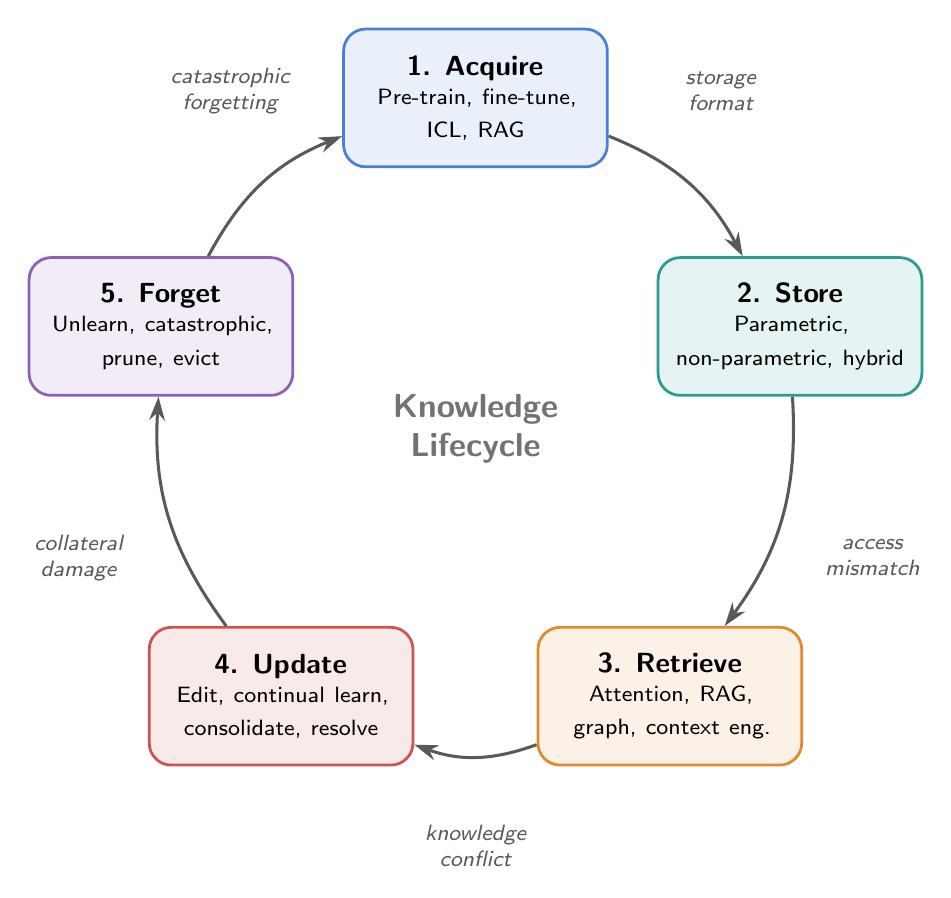
\begin{tikzpicture}[
  % Hyphenation off, and 3.0 cm of measure holds every stage's longest line. The
  % 1.75 cm height floor is what Store and Forget need at four lines, so all five
  % boxes come out the same size.
  stage/.style={
    draw, rounded corners=8pt, minimum width=3.35cm, text width=3.0cm,
    minimum height=1.75cm, font=\sffamily, align=center, line width=1pt,
    execute at begin node={\hyphenpenalty=10000\exhyphenpenalty=10000}
  },
  flow/.style={-{Stealth[length=3mm,width=2mm]}, line width=1.1pt, color=black!65},
  edgelabel/.style={font=\sffamily\footnotesize\itshape, text=black!65,
                    align=center, inner sep=1pt}
]


\def\R{4.2}   % stage centres
\def\L{5.3}   % boundary labels

% --- the five stages, clockwise from the top ---------------------------------
\node[stage, draw=acquire,  fill=acquire!12]  (acq) at ( 90:\R)
  {\textbf{1. Acquire}\\[1pt]{\footnotesize Pre-train, fine-tune,\\ ICL, RAG}};
\node[stage, draw=store,    fill=store!12]    (sto) at ( 18:\R)
  {\textbf{2. Store}\\[1pt]{\footnotesize Parametric,\\ non-parametric, hybrid}};
\node[stage, draw=retrieve, fill=retrieve!12] (ret) at (-54:\R)
  {\textbf{3. Retrieve}\\[1pt]{\footnotesize Attention, RAG,\\ graph, context eng.}};
\node[stage, draw=update,   fill=update!12]   (upd) at (-126:\R)
  {\textbf{4. Update}\\[1pt]{\footnotesize Edit, continual learn,\\ consolidate, resolve}};
\node[stage, draw=forget,   fill=forget!12]   (fgt) at (162:\R)
  {\textbf{5. Forget}\\[1pt]{\footnotesize Unlearn, catastrophic,\\ prune, evict}};

% --- one arc per boundary, bending outward so the ring reads as a cycle -------
\draw[flow] (acq) to[bend left=20] (sto);
\draw[flow] (sto) to[bend left=20] (ret);
\draw[flow] (ret) to[bend left=20] (upd);
\draw[flow] (upd) to[bend left=20] (fgt);
\draw[flow] (fgt) to[bend left=20] (acq);

% --- what goes wrong at each boundary, on the bisector, outside the ring ------
\node[edgelabel] at ( 54:\L) {storage\\format};
\node[edgelabel] at (-18:\L) {access\\mismatch};
\node[edgelabel] at (-90:\L) {knowledge\\conflict};
\node[edgelabel] at (198:\L) {collateral\\damage};
\node[edgelabel] at (126:\L) {catastrophic\\forgetting};

% --- hub ---------------------------------------------------------------------
\node[font=\sffamily\large\bfseries, text=black!55, align=center] at (0,0)
  {Knowledge\\Lifecycle};

\end{tikzpicture}
\caption{The Knowledge Lifecycle framework. Knowledge moves clockwise through five stages, each studied by a distinct research community. The italic label on each boundary names what goes wrong when two adjacent stages disagree, following the cross-stage dependencies of \S\ref{sec:framework}: acquisition dictates storage format, retrieval must match that format, a fact edited in one store but not the other produces a knowledge conflict, every edit is a small forgetting event with collateral damage, and forgetting feeds back into acquisition as catastrophic forgetting. The stages are well covered in isolation; the five boundaries between them are where the open problems lie, and the failure measured in \S\ref{sec:crossmodel} sits on the Retrieve--Update boundary.}
\label{fig:lifecycle}
\end{figure*}

\subsection{Overview of the Five Stages}

\paragraph{Stage 1: Acquisition.} Knowledge enters the system. Pre-training compresses billions of web pages into parameters~\citep{kaplan2020scaling, hoffmann2022chinchilla}. Fine-tuning injects specialized task or domain knowledge~\citep{hu2022lora}. In-context learning supplies knowledge transiently through demonstrations placed in the prompt~\citep{min2022rethinking}. Retrieval-augmented pre-training (REALM~\citep{guu2020realm}, Atlas~\citep{izacard2023atlas}) teaches the model to pull in external text during training itself.

\paragraph{Stage 2: Storage.} Acquired knowledge has to live somewhere. We identify four storage modalities: \textit{parametric} (baked into weights), \textit{non-parametric} (sitting in a vector database, knowledge graph, or document index), \textit{hybrid} (architectures such as RETRO~\citep{borgeaud2022retro} and nearest-neighbor language models~\citep{khandelwal2020knnlm} that blend both), and \textit{agent memory hierarchies} (tiered systems with working, episodic, and archival layers~\citep{packer2023memgpt}).

\paragraph{Stage 3: Retrieval.} A question arrives. The system must locate the right knowledge and bring it to bear. Internal retrieval works through the self-attention mechanism. External retrieval is the RAG pipeline: encode the query, search the index, return the top passages~\citep{karpukhin2020dpr}; graph-structured variants extend it from passage lookup to corpus-level summarization~\citep{edge2024graphrag}. Context engineering, meaning the choice of which passages to include, in what order, and in what format, determines whether retrieved knowledge reaches the model's reasoning process~\citep{liu2024lost}.

\paragraph{Stage 4: Update.} The world changes, and the system's knowledge must change with it. Knowledge editing rewrites individual facts in the weights~\citep{meng2022rome, meng2023memit}. Continual learning extends the model to new domains over time~\citep{kirkpatrick2017ewc}. Agent memory consolidation turns raw interaction logs into distilled insights~\citep{park2023generative}. Knowledge conflict resolution decides what to do when the weights say one thing and the retrieved document says another~\citep{xie2024conflicts, longpre2021entity}.

\paragraph{Stage 5: Forgetting.} Knowledge leaves the system, on purpose or by accident. Machine unlearning removes specific facts to comply with privacy law~\citep{jang2023unlearning, maini2024tofu}. Catastrophic forgetting destroys old knowledge as a side effect of learning new knowledge~\citep{kirkpatrick2017ewc, luo2023catastrophic}. Selective pruning trims bloated agent memory stores. KV-cache eviction drops tokens that no longer fit in the context window~\citep{xiao2024streamingllm}.

\subsection{Cross-Stage Dependencies}

The five stages are not a linear pipeline. They interact, and those interactions create problems that no single stage can solve alone:

\begin{itemize}[leftmargin=*]
  \item \textbf{Acquisition $\leftrightarrow$ Storage.} How knowledge is acquired dictates where it ends up. Pre-training stores knowledge parametrically; RAG stores it externally. This choice echoes through every later stage.
  \item \textbf{Storage $\leftrightarrow$ Retrieval.} Parametric storage relies on implicit retrieval through attention. Non-parametric storage requires an explicit search pipeline. The retrieval mechanism must match the storage format.
  \item \textbf{Retrieval $\leftrightarrow$ Update.} Editing a fact in the weights does not edit it in the vector database, and vice versa. When the two copies disagree, the system produces contradictory outputs.
  \item \textbf{Update $\leftrightarrow$ Forgetting.} Every edit is a small forgetting event: the old fact is overwritten. Every unlearning operation risks collateral damage to neighboring facts. The two problems share root causes.
  \item \textbf{Forgetting $\leftrightarrow$ Acquisition.} Catastrophic forgetting during continual training and deliberate unlearning for privacy are studied by different communities, but both reduce to the same question: how to selectively remove information from entangled representations.
\end{itemize}

% ============================================================
\section{Formalizing the Legacy Pipeline}
\label{sec:legacy_pipeline}
\label{sec:retrieval}
% ============================================================

Before examining how inference-time scaling alters the lifecycle, we formally define the constraints of the Acquisition, Storage, and Retrieval stages. These stages set the baseline mathematics of LLM knowledge management before reasoning models.

\subsection{Acquisition and Parametric Storage}
\label{sec:acquisition}
\label{sec:storage}

Pre-training and fine-tuning serve as the primary mechanisms for eager knowledge acquisition. Autoregressive language models learn by maximum likelihood: the model compresses factual, linguistic, and procedural information into its weights by minimizing the cross-entropy loss over a training corpus $\mathcal{D}$:
\begin{equation}
  \label{eq:ce}
  \mathcal{L}_{\text{CE}}(\theta) = -\mathbb{E}_{x \sim \mathcal{D}} \left[ \sum_{t=1}^T \log P_\theta(x_t \mid x_{<t}) \right]
\end{equation}

\paragraph{Intuition.} This is a mimicry objective. The model predicts the next token in a sequence and receives a penalty when its prediction deviates from the ground truth. The comparison with adversarially trained generators locates the problem in the objective rather than in the architecture: there a second network supplies the learning signal~\citep{thakur2021gan}, and a second network is somewhere information about the source could in principle be carried, whereas Equation~\ref{eq:ce} sees only the next token over an undifferentiated corpus. The process forces factual knowledge into the parameters $\theta$, but it does so without any metadata: the model learns \textit{what} is true, but not \textit{when} or \textit{why} it is true. This absence of provenance is the root cause of the failures analyzed in \S\ref{sec:contributions}.

Once acquired, this knowledge resides implicitly within the feed-forward networks (FFNs). Nothing in the construction of a dense layer~\citep{thakur2021fundamentals} marks it as a memory: it is a weight matrix, a bias, and a nonlinearity, with no field in which to record anything about the data that shaped it. The memory reading is emergent. \citet{geva2021kv} established that Transformer FFNs operate as associative key-value memories. For an input representation $x$, the FFN computation is:
\begin{equation}
  \label{eq:ffn}
  \text{FFN}(x) = f(x K^\top)V = \sum_{i=1}^{d_m} f(x \cdot k_i)\, v_i
\end{equation}
where $k_i$ acts as a key detecting a specific semantic pattern, and $v_i$ acts as a value inducing a corresponding distribution over the output vocabulary.

\paragraph{Intuition.} The FFN behaves as a large, fuzzy look-up table. The keys $k_i$ are concepts the model has memorized, and the values $v_i$ are the answers associated with those concepts. When the input $x$ matches a key (high dot product $x \cdot k_i$), the model recalls the corresponding answer. The difficulty is that these keys and values are entangled across billions of parameters, which makes it nearly impossible to surgically delete or update a single fact without affecting others~\citep{yao2023editingsurvey}.

\subsection{Retrieval-Augmented Constraints}

To bypass the rigidity of parametric storage, the field adopted Retrieval-Augmented Generation~\citep{lewis2020rag}. RAG decouples knowledge storage from the model parameters by maintaining a non-parametric external index. Retrieval is typically framed as a Maximum Inner Product Search (MIPS) over a bi-encoder space~\citep{karpukhin2020dpr}:
\begin{equation}
  d^* = \arg\max_{d \in \mathcal{C}} \left( E_Q(q)^\top E_D(d) \right)
\end{equation}

External retrieval solves the immutability problem of parametric weights, but it introduces a bottleneck of its own. When the retriever injects documents into the context window, the knowledge must pass through the model's self-attention mechanism. If the retrieved context contradicts the model's confident parametric weights, standard forward-pass decoding lacks a formal mechanism to resolve the conflict, and the outcome is unpredictable~\citep{xie2024conflicts, longpre2021entity}. Our measurements in \S\ref{sec:case_study} quantify exactly this failure.

% ============================================================
\section{Update: From Static Editing to Test-Time Resolution}
\label{sec:update}
% ============================================================

\subsection{Static Parameter Modification and Its Limits}

The field first approached knowledge updating through static parameter modification. Early work framed editing as learned constrained optimization over the weights~\citep{decao2021editing}; ROME~\citep{meng2022rome} and MEMIT~\citep{meng2023memit} rewrite specific factual associations in the FFN weights through rank-one and mass edits; MEND~\citep{mitchell2022mend} learns an editing network; SERAC~\citep{mitchell2022serac} routes around the base model with an external edit memory; Transformer-Patcher~\citep{huang2023patcher} and PMET~\citep{li2024pmet} refine the locality of the intervention; task arithmetic composes whole edit directions in weight space~\citep{ilharco2023task}. Across this line of work a consistent limitation emerged, known as the specificity bottleneck: altering a single fact perturbs entangled neighbor representations, and edit quality degrades as edits accumulate~\citep{yao2023editingsurvey}.

\subsection{Representation Engineering and Activation Steering}

An alternative line of work controls behavior without permanently modifying weights. Representation Engineering (RepE)~\citep{zou2023repe} monitors and steers internal activations at inference time: a steering vector added to or gated over the residual stream biases generation away from an undesired direction while the base weights remain intact. Applied to the knowledge lifecycle, steering offers a path around the specificity bottleneck. When a conflict between a retrieved document and a parametric memory is detected, the system can suppress the stale parametric activation for the duration of the query instead of destructively editing it.

\subsection{Test-Time Compute and Conflict Resolution}

Reasoning models trained with reinforcement learning, such as OpenAI o1~\citep{openai2024o1} and DeepSeek-R1~\citep{guo2025deepseekr1}, allocate extended test-time compute to search, reflect, and self-correct before answering. In the lifecycle view, this changes where the Update stage can act: conflicts no longer need to be resolved in a single forward pass, because the model can evaluate competing continuations during its reasoning trajectory. The open question is what signal the model should use to score those continuations. Without metadata recording when and where a parametric fact was acquired, even an extended search has no principled basis for preferring a freshly retrieved fact over a confident but outdated parametric one~\citep{xie2024conflicts}. Supplying exactly this signal is the purpose of the Provenance Vector (\S\ref{sec:contributions}).

% ============================================================
\section{Forgetting}
\label{sec:forgetting}
% ============================================================

\subsection{Machine Unlearning}

Machine unlearning attempts to remove specific data points from the weights, often to comply with privacy regulations~\citep{jang2023unlearning}. Standard approaches apply gradient ascent on the forget-set or fine-tune on obfuscated targets~\citep{eldan2023harrypotter}. Evaluations on benchmarks such as TOFU~\citep{maini2024tofu} show the same entanglement problem seen in editing: aggressive unlearning inflicts collateral damage on retained knowledge, while conservative unlearning leaves the target recoverable through indirect queries. Training-data extraction attacks~\citep{carlini2021extraction} supply the adversarial standard against which unlearning must be verified.

\subsection{Structural Forgetting}

The most routine form of forgetting is structural: context window eviction. Despite advances in streaming attention~\citep{xiao2024streamingllm} and selective state-space models~\citep{gu2023mamba}, active context is bounded, and when an agent's memory stream exceeds it, tokens are dropped. Agent memory hierarchies such as MemGPT~\citep{packer2023memgpt} mitigate this by paging critical information back into active context, which transforms structural forgetting into a recursive retrieval problem. Catastrophic forgetting during continual training~\citep{kirkpatrick2017ewc, luo2023catastrophic} completes the picture: knowledge can leave the system as an unintended side effect of acquisition itself.

% ============================================================
\section{Cross-Cutting Analysis}
\label{sec:analysis}
% ============================================================

\begin{figure}[t]
\centering
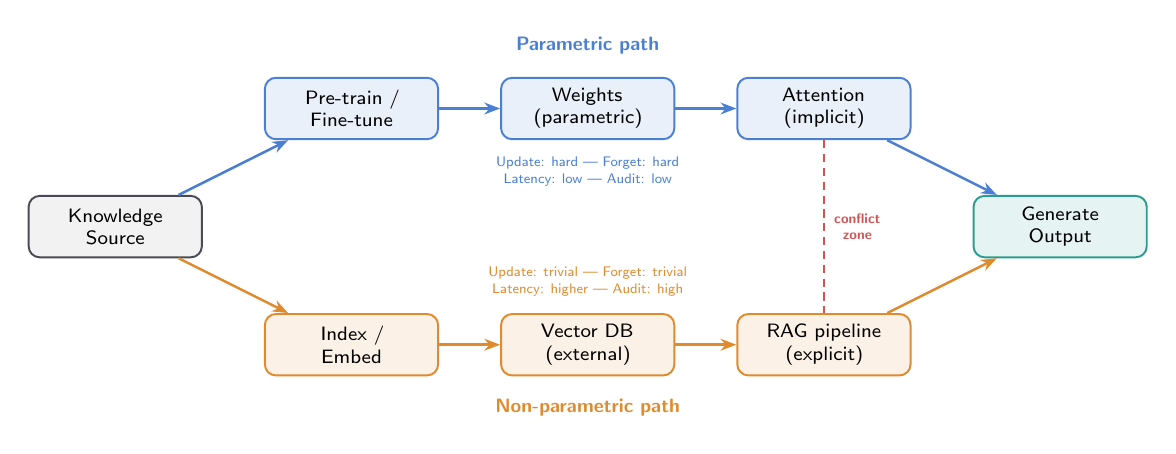
\begin{tikzpicture}[
  % Parametric path in the Acquire blue, non-parametric in the Retrieve orange.
  % The height floor sits above what any box needs, so all eight match.
  box/.style={draw, rounded corners=4pt, minimum width=2.2cm, minimum height=0.78cm,
              text width=1.95cm, font=\sffamily\scriptsize, align=center,
              line width=0.7pt,
              execute at begin node={\hyphenpenalty=10000\exhyphenpenalty=10000}},
  parrow/.style={-{Stealth[length=2mm]}, line width=0.9pt, color=acquire},
  nparrow/.style={-{Stealth[length=2mm]}, line width=0.9pt, color=retrieve},
  plabel/.style={font=\sffamily\scriptsize\bfseries, color=acquire},
  nlabel/.style={font=\sffamily\scriptsize\bfseries, color=retrieve},
  % Property lines at full hue; tinted they print as a smudge.
  pprop/.style={font=\sffamily\tiny, text=acquire, align=center},
  nprop/.style={font=\sffamily\tiny, text=retrieve, align=center}
]

% --- Left: Knowledge source ---
\node[box, draw=muted, fill=black!5] (src) at (0,0) {Knowledge\\Source};

% --- Parametric path (top) ---
\node[box, draw=acquire, fill=acquire!12] (ptrain) at (3, 1.5) {Pre-train /\\Fine-tune};
\node[box, draw=acquire, fill=acquire!12] (pstore) at (6, 1.5) {Weights\\(parametric)};
\node[box, draw=acquire, fill=acquire!12] (pret)   at (9, 1.5) {Attention\\(implicit)};

% --- Non-parametric path (bottom) ---
\node[box, draw=retrieve, fill=retrieve!12] (nindex) at (3, -1.5) {Index /\\Embed};
\node[box, draw=retrieve, fill=retrieve!12] (nstore) at (6, -1.5) {Vector DB\\(external)};
\node[box, draw=retrieve, fill=retrieve!12] (nret)   at (9, -1.5) {RAG pipeline\\(explicit)};

% --- Merge point ---
\node[box, draw=store, fill=store!12] (gen) at (12, 0) {Generate\\Output};

% --- Parametric arrows ---
\draw[parrow] (src) -- (ptrain);
\draw[parrow] (ptrain) -- (pstore);
\draw[parrow] (pstore) -- (pret);
\draw[parrow] (pret) -- (gen);

% --- Non-parametric arrows ---
\draw[nparrow] (src) -- (nindex);
\draw[nparrow] (nindex) -- (nstore);
\draw[nparrow] (nstore) -- (nret);
\draw[nparrow] (nret) -- (gen);

% --- Conflict zone ---
% The Update red, the colour this conflict carries throughout.
\draw[densely dashed, update, line width=0.8pt] (pret) -- (nret)
  node[midway, right, font=\sffamily\tiny\bfseries, text=update, align=center] {conflict\\zone};

% --- Path labels ---
\node[plabel] at (6, 2.3) {Parametric path};
\node[nlabel] at (6, -2.3) {Non-parametric path};

% --- Properties ---
\node[pprop] at (6, 0.7) {Update: hard | Forget: hard\\Latency: low | Audit: low};
\node[nprop] at (6, -0.7) {Update: trivial | Forget: trivial\\Latency: higher | Audit: high};

\end{tikzpicture}
\caption{Two paths through the knowledge lifecycle. The parametric path (top, blue) bakes knowledge into weights during training; it is fast at inference but hard to update or forget. The non-parametric path (bottom, orange) stores knowledge externally; it is easy to modify but depends on retrieval quality. When both paths are active, the ``conflict zone'' (dashed red) produces the knowledge conflict problem discussed in \S\ref{sec:update}.}
\label{fig:two_paths}
\end{figure}

\subsection{Systematic Coverage Analysis of the Literature}

To substantiate the claim that existing work is fragmented, we conducted a systematic mapping of representative publications to the lifecycle stages they address. Table~\ref{tab:coverage} presents this analysis. A checkmark indicates that the paper makes a direct methodological or empirical contribution to that stage; a dash indicates no coverage.

\begin{table*}[t]
\centering
\caption{Literature coverage across lifecycle stages. Each row maps a representative work to the stages it addresses. The rightmost column counts the number of stages covered. The concentration of single- and two-stage papers confirms that the field operates in silos; cross-stage interactions remain largely unstudied.}
\label{tab:coverage}
\small
\begin{tabular}{@{}lcccccr@{}}
\toprule
\textbf{Representative Work} & \textbf{Acquire} & \textbf{Store} & \textbf{Retrieve} & \textbf{Update} & \textbf{Forget} & \textbf{Stages} \\
\midrule
Lewis et al.\ (RAG, 2020) & -- & -- & \checkmark & -- & -- & 1 \\
Karpukhin et al.\ (DPR, 2020) & -- & -- & \checkmark & -- & -- & 1 \\
Meng et al.\ (ROME, 2022) & -- & \checkmark & -- & \checkmark & -- & 2 \\
Meng et al.\ (MEMIT, 2023) & -- & \checkmark & -- & \checkmark & -- & 2 \\
Mitchell et al.\ (SERAC, 2022) & -- & \checkmark & -- & \checkmark & -- & 2 \\
Kirkpatrick et al.\ (EWC, 2017) & \checkmark & -- & -- & \checkmark & \checkmark & 3 \\
Jang et al.\ (Knowledge Unlearning, 2023) & -- & -- & -- & -- & \checkmark & 1 \\
Maini et al.\ (TOFU, 2024) & -- & -- & -- & -- & \checkmark & 1 \\
Borgeaud et al.\ (RETRO, 2022) & \checkmark & \checkmark & \checkmark & -- & -- & 3 \\
Guu et al.\ (REALM, 2020) & \checkmark & -- & \checkmark & -- & -- & 2 \\
Izacard et al.\ (Atlas, 2023) & \checkmark & -- & \checkmark & -- & -- & 2 \\
Park et al.\ (Generative Agents, 2023) & \checkmark & \checkmark & \checkmark & \checkmark & \checkmark & 5 \\
Packer et al.\ (MemGPT, 2023) & -- & \checkmark & \checkmark & \checkmark & \checkmark & 4 \\
Xie et al.\ (Knowledge Conflicts, 2024) & -- & \checkmark & \checkmark & \checkmark & -- & 3 \\
Hu et al.\ (LoRA, 2022) & \checkmark & \checkmark & -- & -- & -- & 2 \\
Kaplan et al.\ (Scaling Laws, 2020) & \checkmark & -- & -- & -- & -- & 1 \\
Khandelwal et al.\ (kNN-LM, 2020) & -- & \checkmark & \checkmark & -- & -- & 2 \\
Carlini et al.\ (Data Extraction, 2021) & -- & \checkmark & -- & -- & \checkmark & 2 \\
Luo et al.\ (Catastrophic Forgetting, 2023) & \checkmark & -- & -- & -- & \checkmark & 2 \\
Edge et al.\ (GraphRAG, 2024) & -- & \checkmark & \checkmark & -- & -- & 2 \\
\midrule
\textbf{This paper} & \checkmark & \checkmark & \checkmark & \checkmark & \checkmark & \textbf{5} \\
\bottomrule
\end{tabular}
\end{table*}

Of the 20 representative works mapped, 5 address only a single lifecycle stage, 10 address exactly two, 3 address three, and only 2 (Generative Agents and MemGPT) touch four or more. The median coverage is 2 stages. No prior work provides a unified formalism across all five. Pairwise coverage is thinner still. Counting how often two stages are addressed by the same work, the Acquisition--Update and Retrieval--Forgetting pairs are the least studied at 2 works each, and the Acquisition--Forgetting and Update--Forgetting pairs follow at 3, the last two despite being the source of damaging real-world failures such as fine-tuning that silently overwrites earlier alignment. The two most studied pairs, Storage--Retrieval and Storage--Update at 6 works each, are precisely the ones that sit inside an established subfield rather than across two.

\subsection{Parametric vs.\ Non-Parametric: A Unified View}

The first design decision in any LLM knowledge system is where the knowledge goes: into the weights or outside them. Figure~\ref{fig:two_paths} visualizes the two paths, and Table~\ref{tab:parametric_comparison} lays out how this choice plays out across every lifecycle stage.

\begin{table}[t]
\centering
\caption{How the parametric/non-parametric choice affects each lifecycle stage.}
\label{tab:parametric_comparison}
\small
\begin{tabular}{@{}lll@{}}
\toprule
\textbf{Lifecycle Stage} & \textbf{Parametric} & \textbf{Non-Parametric} \\
\midrule
Acquisition & Pre-training, fine-tuning & Indexing documents \\
Storage & Distributed in weights & Explicit in databases \\
Retrieval & Attention (implicit) & Search pipeline (explicit) \\
Update & Knowledge editing (hard) & Database write (trivial) \\
Forgetting & Unlearning (hard) & Delete entry (trivial) \\
\midrule
Latency & Low (single forward pass) & Higher (retrieval + generation) \\
Auditability & Low (opaque weights) & High (traceable sources) \\
Scalability & Fixed at training time & Grows with corpus \\
\bottomrule
\end{tabular}
\end{table}

Parametric storage is fast and tightly integrated with the model's reasoning, but opaque, rigid, and difficult to modify. Non-parametric storage is modular and transparent, but depends on the retrieval pipeline surfacing the right knowledge at the right time. A lifecycle-aware hybrid takes both: route stable, frequently accessed knowledge into the weights, and dynamic, auditable, regulation-sensitive knowledge into external stores, where it can be updated and deleted without touching the model.

\subsection{Evaluation Methods and Benchmarks}

Every lifecycle stage has its own evaluation protocol, and none of them accounts for the others. RAG systems measure retrieval recall and end-to-end answer quality~\citep{es2024ragas, chen2024benchmarking}. Knowledge editing measures efficacy, specificity, and generalization~\citep{yao2023editingsurvey}. Unlearning measures whether the target knowledge can be extracted through membership inference and extraction attacks~\citep{maini2024tofu, carlini2021extraction}. Agent memory systems are beginning to use multi-session benchmarks that test whether an agent can recall information from many conversations ago~\citep{hu2025agentmemory}.

The gap is structural. A system can score well on a RAG benchmark and a knowledge editing benchmark individually, while failing when the two stages interact, for example when an edited fact is overridden by a stale retrieved passage. What the field needs is a lifecycle benchmark: a test suite that evaluates a sequence of operations (store, retrieve, update, verify the update, forget, verify the deletion) on the same set of facts. No such benchmark exists today.

\subsection{The Knowledge Consistency Problem}

The hardest cross-stage problem is consistency. As knowledge flows through the lifecycle, inconsistencies accumulate from at least four sources:

\begin{itemize}[leftmargin=*]
  \item \textbf{Temporal.} The weights reflect the training cutoff. The retrieved documents reflect the current date. The model may blend the two, producing an answer that is partly outdated and partly current.
  \item \textbf{Source-level.} Two retrieved documents may contradict each other. The model has no mechanism to determine which source is more reliable.
  \item \textbf{Edit-level.} An edit changes ``The capital of Country X is A'' to ``The capital of Country X is B,'' but leaves all related facts (``A is the largest city in Country X'') unchanged. The model's knowledge is now internally contradictory.
  \item \textbf{Forgetting-level.} An unlearning operation removes a fact when asked directly, but the model can still reconstruct it from indirect cues. The fact is technically forgotten but practically recoverable.
\end{itemize}

Consistency is a lifecycle problem by definition. It cannot be fixed at any single stage. Fixing it requires a provenance system that tracks every fact through every stage: when it was acquired, where it is stored, how it has been retrieved, whether it has been updated, and whether it has been marked for deletion. The next section develops the architectural and metrological components of exactly such a system.

% ============================================================
\section{Original Contributions}
\label{sec:contributions}
% ============================================================

From the five-stage analysis we propose two technical components for the asymmetries the lifecycle creates. Table~\ref{tab:synthesis} summarizes the failure modes identified in the preceding sections and the corresponding mechanisms introduced here.

\begin{table}[h]
\centering
\caption{Synthesis of Knowledge Lifecycle failure modes and the mechanisms proposed in this work.}
\label{tab:synthesis}
\small
\begin{tabular}{@{}llll@{}}
\toprule
\textbf{Stage} & \textbf{Primary Failure Mode} & \textbf{Root Cause} & \textbf{Proposed Mechanism} \\ \midrule
Acquisition & Entanglement & Metadata-free compression & Provenance Vector ($p$) \\
Storage & Boundary conflict & Parametric/non-parametric gap & Metric: $\mathcal{D}_{sync}$ \\
Retrieval & Context override failure & Static forward-pass priority & Provenance-aware scoring \\
Update & Specificity bottleneck & Destructive weight modification & Activation gating \\
Forgetting & Collateral damage & Gradient-based unlearning & Gate-level suppression \\ \bottomrule
\end{tabular}
\end{table}

\subsection{Architectural Proposal: The Provenance Vector ($p$)}
\label{sec:provenance}

Transformers store facts implicitly as key-value pairs in FFNs (\S\ref{sec:storage}). When knowledge conflicts arise (\S\ref{sec:update}), the network has no mathematical basis for prioritizing one fact over another, because provenance, meaning when and from where the fact was acquired, is discarded during parametric compression.

We propose extending each FFN memory slot from a pair $(k_i, v_i)$ to a triple $(k_i, v_i, p_i)$, where the \textit{Provenance Vector} $p_i \in \mathbb{R}^{d_p}$ is a learned embedding of the acquisition timestamp $\tau_i$ and a source reliability score $s_i$:
\begin{equation}
  p_i = E_p([\tau_i \,;\, s_i]), \qquad E_p : \mathbb{R}^2 \to \mathbb{R}^{d_p}
\end{equation}
The provenance store is metadata: it does not enter the residual stream and therefore leaves the dimensionality and function of the standard FFN untouched. Its sole consumer is a gating function evaluated during inference (\S\ref{sec:gating}).

\paragraph{Training objective.} During pre-training, an auxiliary loss trains the provenance store. Given a training example drawn from source $s$ at timestamp $\tau$, the model minimizes a joint objective:
\begin{equation}
  \mathcal{L}_{total} = \mathcal{L}_{\text{CE}}(\theta) + \alpha \cdot \mathcal{L}_{prov}
\end{equation}
where $\mathcal{L}_{prov}$ is a Mean Squared Error (MSE) regression loss between a decoding of the provenance embeddings of the activated slots and the ground-truth metadata $[\tau; s]$ of the example, and $\alpha$ balances the two objectives. Slots that activate strongly on an example are pushed to carry that example's provenance; slots activated by many temporally scattered examples learn an averaged timestamp with correspondingly lower reliability, which is itself informative.

\paragraph{Complexity.} The modification adds $d_p$ dimensions to each of the $d_m$ slots per FFN layer. Setting $d_p = 8$ on a 32-layer model with $d_m = 4096$ adds $8 \times 4096 \times 32 \approx 1.05$M parameters, below $0.02\%$ of a 7B-parameter model. Inference cost grows by one elementwise gate per FFN slot, which is negligible relative to the matrix products in Equation~\ref{eq:ffn}.

\subsection{Provenance-Gated Inference}
\label{sec:gating}

At inference time, let $T_{now}$ be the current timestamp and $\Delta\tau_i = T_{now} - \tau_i \geq 0$ the age of slot $i$. We define a gate $S(\Delta\tau_i) \in (0, 1)$ over each slot, using a sigmoidal soft threshold; soft membership functions of this kind have long been used to blend symbolic thresholds with continuous activations in neuro-fuzzy systems~\citep{thakur2021neurofuzzy}:
\begin{equation}
  \label{eq:gate}
  S(\Delta\tau_i) = \sigma\!\left( \gamma - \beta \cdot \Delta\tau_i \right)
  = \frac{1}{1 + \exp\!\left(\beta \cdot \Delta\tau_i - \gamma\right)}
\end{equation}
where $\beta > 0$ is a learned sensitivity parameter and $\gamma > 0$ is a freshness threshold. The gate decreases monotonically with age: fresh slots ($\Delta\tau_i \approx 0$) pass with $S \approx \sigma(\gamma) \approx 1$, while stale slots are attenuated. The steered FFN computation becomes the following, with the full forward pass stated as Algorithm~\ref{alg:gated_ffn}:
\begin{equation}
  \label{eq:steering}
  \text{FFN}_{steered}(x) = \sum_{i=1}^{d_m} S(\Delta\tau_i)\, f(x \cdot k_i)\, v_i
\end{equation}

\paragraph{Adaptive thresholding.} The threshold $\gamma$ need not be static. A reasoning model can compute it during its reflection loop from the entropy of its own predictive distribution: when the model detects a conflict between context and parametric prediction (high entropy or divergent candidate continuations), it lowers $\gamma$, making the gate more aggressive for that query. This couples the gate to test-time compute: more deliberation buys sharper conflict resolution, without any weight modification.

\paragraph{Intuition.} The gate is a volume control attached to every fact in the model's memory. A fact's age turns its volume down; the query's difficulty decides how strict the ceiling is. An outdated fact that contradicts a fresh retrieved document is attenuated at its source, inside the FFN sum, before it can pollute the residual stream. The base weights are never modified, so there is no collateral damage of the kind that limits static editing (\S\ref{sec:update}).

\begin{algorithm}[t]
\caption{Provenance-gated FFN forward pass}
\label{alg:gated_ffn}
\begin{algorithmic}[1]
\Require input representation $x$; slots $\{(k_i, v_i, p_i)\}_{i=1}^{d_m}$; current time $T_{now}$; sensitivity $\beta$; threshold $\gamma$
\Ensure steered FFN output $o$
\State $o \gets \mathbf{0}$
\For{$i = 1$ to $d_m$}
  \State $a_i \gets f(x \cdot k_i)$ \Comment{standard key activation}
  \If{$a_i \neq 0$}
    \State $(\tau_i, s_i) \gets \text{decode}(p_i)$ \Comment{read metadata, not the residual stream}
    \State $\Delta\tau_i \gets T_{now} - \tau_i$
    \State $g_i \gets \sigma(\gamma - \beta \cdot \Delta\tau_i)$ \Comment{Equation~\ref{eq:gate}}
    \State $o \gets o + g_i \cdot a_i \cdot v_i$
  \EndIf
\EndFor
\State \Return $o$
\end{algorithmic}
\end{algorithm}

\subsection{Idealized Consistency Analysis}
\label{sec:analysis_proof}

We now state the conditions under which provenance gating provably resolves a parametric-contextual conflict. The result is an idealized analysis, not a guarantee about production systems; its purpose is to show that the mechanism is structurally sound, and its assumptions make explicit what a real implementation must approximate.

\begin{assumption}
\label{as:stale_support}
There exists a threshold $\tau^{\ast} > 0$ such that, for query $q$, every FFN slot whose value vector contributes to the outdated answer has age $\Delta\tau_i > \tau^{\ast}$, and every slot contributing to other necessary computation (syntax, style, task format) has age $\Delta\tau_i < \tau^{\ast}$.
\end{assumption}

\begin{assumption}
\label{as:context_sufficiency}
The retrieved context $\mathcal{M}_{now}$ contains the updated fact, and with the conflicting parametric contribution suppressed, the model's output distribution on $q$ is determined by attention over $\mathcal{M}_{now}$; denote this distribution $P_{ctx}(y \mid q, \mathcal{M}_{now})$.
\end{assumption}

\begin{proposition}
\label{prop:consistency}
Under Assumptions~\ref{as:stale_support} and \ref{as:context_sufficiency}, and with the freshness threshold tied to the sensitivity as $\gamma = \beta\tau^{\ast}$ so that the gate's decision boundary stays at $\tau^{\ast}$ while the gate sharpens, the gated model's output distribution converges to $P_{ctx}$ as $\beta \to \infty$, and consequently
\begin{equation}
  \lim_{\beta \to \infty} D_{KL}\!\left( P_{ctx} \,\|\, P_{steered} \right) = 0.
\end{equation}
\end{proposition}

\begin{proof}
Equation~\ref{eq:gate} places the gate's decision boundary at $\Delta\tau_i = \gamma/\beta$, so the coupling $\gamma = \beta\tau^{\ast}$ fixes that boundary at $\tau^{\ast}$ and reduces the gate to $S(\Delta\tau_i) = \sigma\!\left(\beta(\tau^{\ast} - \Delta\tau_i)\right)$. For a slot with $\Delta\tau_i > \tau^{\ast}$ the argument $\beta(\tau^{\ast} - \Delta\tau_i) \to -\infty$ as $\beta \to \infty$, so $S(\Delta\tau_i) \to 0$; for a slot with $\Delta\tau_i < \tau^{\ast}$ the argument tends to $+\infty$ and $S \to 1$. The gate therefore converges pointwise to the indicator $\mathbf{1}\!\left[\Delta\tau_i < \tau^{\ast}\right]$. By Assumption~\ref{as:stale_support}, exactly the slots supporting the outdated answer are suppressed in Equation~\ref{eq:steering} while all others pass unchanged. By Assumption~\ref{as:context_sufficiency}, the resulting output distribution is $P_{ctx}$, and $D_{KL}(P_{ctx} \| P_{ctx}) = 0$.

The coupling is what makes the limit meaningful. Sharpening the gate with $\gamma$ held fixed drives the boundary $\gamma/\beta$ to zero, which suppresses every slot of positive age, including the ones Assumption~\ref{as:stale_support} requires to survive; the limit would then describe a model with no FFN contribution at all rather than a model with its stale facts removed.
\end{proof}

The assumptions are strong, and stating them is the point. Assumption~\ref{as:stale_support} requires provenance to separate fact slots from infrastructure slots by age, which real training will achieve only approximately; Assumption~\ref{as:context_sufficiency} requires the retriever to have found the updated fact at all. What the proposition establishes is that, given accurate provenance, conflict resolution reduces to a per-slot gating operation with no weight modification, in contrast to static editing where every update risks the specificity bottleneck.

\subsection{Evaluation Metric: Lifecycle Desynchronization ($\mathcal{D}_{sync}$)}
\label{sec:dsync}

The field currently evaluates lifecycle stages in isolation, which masks cross-stage failures (\S\ref{sec:analysis}). We propose a unified metric, \textit{Lifecycle Desynchronization}, that quantifies the failure occurring when a model's parametric state contradicts its non-parametric state.

\paragraph{Definition.} Let $\theta_{stale}$ be the deployed model's weights, $\mathcal{M}_{now}$ the current external knowledge store, and $P_{sync}(y \mid q)$ the output distribution of a hypothetical fully synchronized system whose weights agree with $\mathcal{M}_{now}$. For a query $q$ probing a fact that changed after the training cutoff:
\begin{equation}
  \label{eq:dsync}
  \mathcal{D}_{sync}(q) = D_{KL}\!\left( P_{sync}(y \mid q) \,\Big\|\, P(y \mid q,\, \theta_{stale},\, \mathcal{M}_{now}) \right)
\end{equation}
A large value means the deployed system, even with the corrective context in its window, produces a distribution far from what a synchronized system would produce: the parametric prior is overriding the context. In the terminology of \citet{xie2024conflicts}, high $\mathcal{D}_{sync}$ is quantified stubbornness; a model that follows the context faithfully scores near zero.

\paragraph{Point-mass estimator.} Equation~\ref{eq:dsync} is not directly measurable, because the synchronized distribution is not observable, but for factual queries with a single verifiable answer $y^*$ it is well approximated by a point mass on $y^*$. The KL divergence from a point mass reduces to a surprisal:
\begin{equation}
  \label{eq:estimator}
  \widehat{\mathcal{D}}_{sync}(q) = D_{KL}\!\left( \delta_{y^*} \,\|\, P \right) = -\ln P\!\left(y^* \mid q,\, \theta_{stale},\, \mathcal{M}_{now}\right)
\end{equation}
This estimator is measurable on any model that exposes token probabilities, requires no retraining or counterfactual model, and is expressed in nats with a direct probabilistic reading: $\widehat{\mathcal{D}}_{sync} = n$ means the deployed system assigns the correct answer probability $e^{-n}$.

\paragraph{Interpretation scale.} Because the estimator is a negative log probability, thresholds carry concrete meaning: $\widehat{\mathcal{D}}_{sync} \leq \ln 2 \approx 0.69$ means the correct answer holds at least half the probability mass; values near $4.6$ mean it has fallen to roughly $1\%$; values above $9.2$ mean below $10^{-4}$, a regime in which greedy decoding never selects the correct answer and sampling reaches it less than once in ten thousand draws. We treat this last regime as desynchronization failure.

\paragraph{Context influence.} A complementary diagnostic separates ignoring the context from lacking the answer: the full-vocabulary divergence between the deployed model's distributions with and without the retrieved context,
\begin{equation}
  \label{eq:influence}
  \mathcal{I}_{ctx}(q) = D_{KL}\!\left( P(y \mid q, \mathcal{M}_{now}) \,\|\, P(y \mid q) \right)
\end{equation}
If $\mathcal{I}_{ctx}$ is small while $\widehat{\mathcal{D}}_{sync}$ is large, the context is present but inert: the model's distribution barely moves when the corrective document is supplied. This pairing localizes the failure to the conflict-resolution boundary rather than the retriever.

\begin{algorithm}[t]
\caption{$\mathcal{D}_{sync}$ measurement protocol}
\label{alg:dsync}
\begin{algorithmic}[1]
\Require model with weights $\theta_{stale}$ and token-probability access; conflict pair (query $q$, correct continuation $y^*$, corrective document $m$)
\Ensure $\widehat{\mathcal{D}}_{sync}$, context influence $\mathcal{I}_{ctx}$
\State $P_0 \gets \text{softmax}\left(\text{logits}(q)\right)$ \Comment{condition A: no context}
\State $P_1 \gets \text{softmax}\left(\text{logits}(m \oplus q)\right)$ \Comment{condition B: corrective context prepended}
\State verify tokenization: $y^*$ must map to a defined token sequence in both conditions
\State $\widehat{\mathcal{D}}_{sync} \gets -\ln P_1(y^*)$ \Comment{Equation~\ref{eq:estimator}}
\State $\mathcal{I}_{ctx} \gets \sum_{y} P_1(y) \ln \left( P_1(y) / P_0(y) \right)$ \Comment{Equation~\ref{eq:influence}}
\State \Return $\widehat{\mathcal{D}}_{sync}$, $\mathcal{I}_{ctx}$, and the top-$k$ tokens of $P_0$, $P_1$ for inspection
\end{algorithmic}
\end{algorithm}

\subsection{Case Study and Measurement: The Vioxx Withdrawal}
\label{sec:case_study}

To demonstrate that lifecycle failures are not hypothetical, we trace a documented pharmaceutical event through all five stages, then measure the resulting desynchronization on a real model. Rofecoxib (marketed as Vioxx), a COX-2 selective inhibitor, was approved by the Food and Drug Administration (FDA) in 1999 and voluntarily withdrawn by Merck in September 2004 after the APPROVe trial revealed an elevated risk of cardiovascular events.

\begin{figure}[h]
\centering
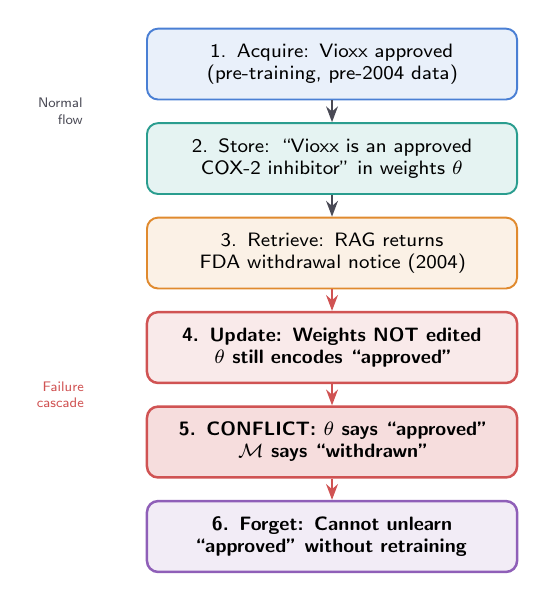
\begin{tikzpicture}[
  % A text width and a height floor, so the six boxes read as one column rather
  % than as a ragged stack. 4.4 cm is set by the longest bold row, which keeps
  % every row to two lines. Hyphenation off so an overlong line shows itself.
  stage/.style={draw, rounded corners=4pt, minimum width=4.7cm, text width=4.4cm,
                minimum height=0.9cm, font=\sffamily\scriptsize, align=center,
                line width=0.7pt,
                execute at begin node={\hyphenpenalty=10000\exhyphenpenalty=10000}},
  % Failing rows are marked by weight and by the red arrows feeding them, not by
  % overriding the stage colour, so the cascade reads stage by stage.
  fail/.style={stage, font=\sffamily\scriptsize\bfseries, line width=0.9pt},
  arr/.style={-{Stealth[length=2mm]}, line width=0.7pt, color=muted},
  farr/.style={-{Stealth[length=2mm]}, line width=0.9pt, color=update}
]

\node[stage, draw=acquire,  fill=acquire!12]  (acq)  at (0,  0)    {1. Acquire: Vioxx approved\\(pre-training, pre-2004 data)};
\node[stage, draw=store,    fill=store!12]    (sto)  at (0, -1.2)  {2. Store: ``Vioxx is an approved\\COX-2 inhibitor'' in weights $\theta$};
\node[stage, draw=retrieve, fill=retrieve!12] (ret)  at (0, -2.4)  {3. Retrieve: RAG returns\\FDA withdrawal notice (2004)};
\node[fail,  draw=update,   fill=update!12]   (upd)  at (0, -3.6)  {4. Update: Weights NOT edited\\$\theta$ still encodes ``approved''};
\node[fail,  draw=update,   fill=update!20]   (conf) at (0, -4.8)  {5. CONFLICT: $\theta$ says ``approved''\\$\mathcal{M}$ says ``withdrawn''};
\node[fail,  draw=forget,   fill=forget!12]   (fgt)  at (0, -6.0)  {6. Forget: Cannot unlearn\\``approved'' without retraining};

\draw[arr] (acq) -- (sto);
\draw[arr] (sto) -- (ret);
\draw[farr] (ret) -- (upd);
\draw[farr] (upd) -- (conf);
\draw[farr] (conf) -- (fgt);

\node[font=\sffamily\tiny, text=muted, align=right] at (-3.45, -0.6) {Normal\\flow};
\node[font=\sffamily\tiny, text=update, align=right] at (-3.45, -4.2) {Failure\\cascade};

\end{tikzpicture}
\caption{A lifecycle failure cascade applied to the Rofecoxib (Vioxx) withdrawal. The parametric weights encode an outdated drug approval from pre-training data (Stages 1--2). The RAG index is updated with the FDA withdrawal notice (Stage 3), but no weight edit is applied (Stage 4). The resulting conflict produces a dangerous output (Stage 5), and cannot be resolved without costly retraining (Stage 6). No single-stage benchmark detects this failure.}
\label{fig:failure_cascade}
\end{figure}

\paragraph{Scenario.} Figure~\ref{fig:failure_cascade} traces the cascade stage by stage. Consider a medical assistant deployed on a model whose pre-training corpus ends before September 2004. The fact ``Rofecoxib (Vioxx) is an FDA-approved COX-2 selective anti-inflammatory drug'' is encoded into the parametric weights during pre-training (Acquisition $\rightarrow$ Storage). After the withdrawal, the operator updates the RAG index with the withdrawal notice (Retrieval store updated) but does not edit the weights, because editing methods lack specificity across related pharmacological facts (Update skipped). A clinician asks whether the drug is safe to prescribe. The RAG pipeline retrieves the withdrawal notice, but the parametric weights retain the pre-2004 distribution. Per \citet{xie2024conflicts}, the outcome of this conflict is unpredictable. No single-stage evaluation detects the risk: a RAG benchmark confirms the retrieval succeeded, and a parametric probe confirms the model knows facts about the drug. The failure exists entirely at the boundary.

\paragraph{Measurement.} We instantiate Algorithm~\ref{alg:dsync} on GPT-2 base (124M parameters)~\citep{radford2019gpt2} under deterministic decoding. The query is \textit{``Question: Is Vioxx safe to prescribe? Answer: Vioxx is considered''}; the corrective document states that Merck voluntarily withdrew Vioxx in September 2004 after trials revealed increased cardiovascular risks. Table~\ref{tab:vioxx_results} reports the results. The measurement script is included in the accompanying repository~\citep{thakur2026code} and is exactly reproducible: it uses greedy analysis of the next-token distribution with no sampling. The same probe can be run without installing anything through the interactive demonstration~\citep{thakur2026demo}.

\begin{table}[h]
\centering
\caption{Next-token probabilities for the Vioxx probe on GPT-2 base, with and without the corrective withdrawal document in context. All values measured; script in the project repository.}
\label{tab:vioxx_results}
\small
\begin{tabular}{@{}lrr@{}}
\toprule
\textbf{Quantity} & \textbf{Without context} & \textbf{With context} \\
\midrule
$P(\text{`` safe''})$ (incorrect) & 37.53\% & 42.58\% \\
$P(\text{`` withdrawn''})$ (correct) & 0.0004\% & 0.0006\% \\
$P(\text{`` unsafe''})$ & 1.26\% & 0.51\% \\
Top-1 token & `` safe'' & `` safe'' \\
\midrule
$\mathcal{I}_{ctx}$ (Equation~\ref{eq:influence}) & \multicolumn{2}{c}{0.033 nats} \\
$\widehat{\mathcal{D}}_{sync}$ (Equation~\ref{eq:estimator}) & \multicolumn{2}{c}{12.05 nats} \\
\bottomrule
\end{tabular}
\end{table}

\paragraph{Findings.} Three observations follow. First, the correct continuation `` withdrawn'' receives probability $5.9 \times 10^{-6}$ even with the withdrawal notice present, placing $\widehat{\mathcal{D}}_{sync} = 12.05$ nats deep in the failure regime: no realistic decoding strategy recovers the correct answer. Second, the context barely moves the model: it shifts the full output distribution by only $\mathcal{I}_{ctx} = 0.033$ nats, so the failure is localized to conflict resolution, not retrieval. Third, the corrective context slightly \textit{increases} the probability of the incorrect answer `` safe'' (37.53\% to 42.58\%) and decreases that of `` unsafe''; merely mentioning the drug in a safety-related passage reinforces the dominant parametric association rather than overriding it. This last effect is a concrete, measurable instance of the failure mode that provenance gating (\S\ref{sec:gating}) is designed to eliminate: the stale parametric activation, not the retrieved evidence, controls the output.

\paragraph{Scope of the measurement.} GPT-2 base is a deliberately small, fully open model: it makes the probe exactly reproducible on commodity hardware and free of instruction-tuning confounds. The measured numbers characterize this model and probe, not frontier systems; \S\ref{sec:crossmodel} carries the same protocol across five further models, including instruction-tuned ones, and finds that this probe does not resolve at any scale tested. The probe establishes that the failure mode exists, that it is measurable, and that the metric separates its two possible causes.


\subsection{Cross-Model Measurement}
\label{sec:crossmodel}

The single-model probe establishes that the failure exists. Whether it survives
scale and instruction tuning is a separate question, and one the metric is built
to answer. We therefore ran the protocol of Algorithm~\ref{alg:dsync} unchanged
across six open models spanning 124M to 1.5B parameters and three documented
fact changes: the Vioxx withdrawal of 2004, the British royal succession of
2022, and the renaming of Twitter to X in 2023. Every model is evaluated in
float32 on identical prompts, with no sampling, so the eighteen measurements
reproduce exactly. Table~\ref{tab:crossmodel} reports them.

\begin{table}[t]
\centering
\caption{Cross-model measurement. $\widehat{\mathcal{D}}_{sync}$ and
$\mathcal{I}_{ctx}$ in nats, both with the corrective document present.
\textbf{Bold} marks the cases where the model's most likely continuation is the
correct answer. Surprisal is summed over every token the answer occupies, so the
values are exact on every tokenizer rather than first-token bounds.}
\label{tab:crossmodel}
\small
\begin{tabular}{lrrrrrrr}
\toprule
& & \multicolumn{3}{c}{$\widehat{\mathcal{D}}_{sync}$ (nats)}
& \multicolumn{3}{c}{$\mathcal{I}_{ctx}$ (nats)} \\
\cmidrule(lr){3-5} \cmidrule(lr){6-8}
Model & Params (M) & Vioxx & Monarch & Twitter & Vioxx & Monarch & Twitter \\
\midrule
GPT-2 base & 124 & 12.05 & 2.91 & 2.09 & 0.03 & 0.16 & 0.90 \\
GPT-2 medium & 355 & 10.96 & \textbf{1.41} & 1.19 & 0.12 & 0.76 & 1.43 \\
GPT-2 large & 774 & 11.91 & 3.99 & \textbf{0.71} & 0.10 & 0.14 & 3.66 \\
Qwen2.5-0.5B-Instruct & 494 & 7.03 & 3.32 & \textbf{0.32} & 0.42 & 0.18 & 7.69 \\
TinyLlama-1.1B-Chat & 1100 & 9.22 & 1.78 & \textbf{0.17} & 0.05 & 2.05 & 7.82 \\
Qwen2.5-1.5B-Instruct & 1544 & 8.85 & \textbf{0.64} & \textbf{0.09} & 0.44 & 2.28 & 3.43 \\
\bottomrule
\end{tabular}
\end{table}

\paragraph{The conflict does not resolve with scale.} No model in the ladder
answers the Vioxx probe correctly. The most likely continuation is \textit{safe} for
all three GPT-2 models and for TinyLlama, and $\widehat{\mathcal{D}}_{sync}$
stays above 7 nats everywhere, so even the best case leaves the correct answer
below one chance in a thousand while the withdrawal notice sits in the prompt.
Scale does not move it monotonically: within the GPT-2 family the value falls
from 12.05 to 10.96 and then rises again to 11.91, so the 774M model is worse at
this probe than the 355M one.

\paragraph{Some conflicts do resolve, which is what makes the metric useful.}
The Twitter probe behaves in the opposite way. Within the GPT-2 family
$\widehat{\mathcal{D}}_{sync}$ falls monotonically with size, from 2.09 to 1.19
to 0.71. It reaches 0.09 at the largest model measured, and every model at 494M
or above answers `` X'' correctly. Ordered by parameter count the six values are
not monotone, because the 494M instruction-tuned model beats the 774M base one;
the within-family column is the comparison that holds size as the only variable. The Monarch probe sits between the two and is
also non-monotone within the GPT-2 family: the 355M model answers `` Charles''
correctly and the 774M model regresses to `` Queen''. A metric that reported
failure everywhere would be measuring its own construction; these three probes
separate cleanly, so the metric tracks the conflict and not the difficulty of
the question.

\paragraph{Attending to the document is not the same as being governed by it.}
$\mathcal{I}_{ctx}$ rises with size on the Twitter probe within the GPT-2
family, from 0.90 to 1.43 to 3.66 nats, and reaches 7.82 at TinyLlama; the
models that move most on this probe are the ones that answer it correctly. On
the Vioxx probe it stays low for every GPT-2 model and for TinyLlama, between
0.03 and 0.12 nats, while the answer stays wrong. The pairing is the point: a large
$\mathcal{I}_{ctx}$ with a large $\widehat{\mathcal{D}}_{sync}$ is a model that
read the document and still lost to its weights, and no single-stage benchmark
distinguishes that from a retriever that failed.

\paragraph{Two controls separate an unreachable answer from an unused document.}
Every probe is additionally run against two controls.
An \textit{irrelevant} document, matched to the corrective one in length
and register, establishes how far any document at all moves the model. A
\textit{leak} document, which states the answer outright, establishes how far the
model can be moved when the answer is handed to it. The gap between the leak and
the corrective condition is help that was available and not taken.

On the Vioxx probe that gap is the result. Stating the answer outright is worth
between 7.7 and 10.6 nats to every model on the ladder, so the correct
continuation is well within reach of all of them. The corrective document, which
contains the same fact in prose, is worth at most 0.41 nats to any GPT-2 model.
The failure is not that the model cannot represent the answer; it is that a
document saying so does not reach it. Figure~\ref{fig:help} shows that gap for
every model and probe. Sharper still, on GPT-2 the irrelevant
document about the Danube moves the output distribution 0.089 nats against the
withdrawal notice's 0.033, and an irrelevant document has the larger effect in
2 of the 18 measurements.

\paragraph{The exposure trap is the common case, not the exception.} Comparing
the surprisal of the \textit{stale} answer with and without the corrective
document, the document makes the stale answer \textit{more} likely on the Vioxx
probe for 5 of the 6 models. Naming a fact, even to correct it,
reinforces the association the model already holds. This is the effect that
\S\ref{sec:case_study} reports for a single model, measured across the ladder.

\paragraph{How much of this is the question, and how much is the wording?} A
surprisal measured on one sentence may be a fact about that sentence, so we
re-ran every probe under two further phrasings that ask the same question in
different words, holding the corrective document and the verified answer fixed.
The wording matters, and by a wide margin. On the Vioxx probe
$\widehat{\mathcal{D}}_{sync}$ has a median standard deviation of 5.14 nats
across the three phrasings, and the phrasing used above is the hardest of the
three for all six models: it averages 10.00 nats where the three-phrasing mean is
4.44. The Monarch and Twitter probes are steadier, at 0.87 and 1.67 nats
respectively.

The likely cause is syntactic rather than semantic. ``Vioxx is
considered~\rule{6mm}{0.4pt}'' invites an adjective, and the verified answer
`` withdrawn'' is a participle that sits awkwardly in that frame, whereas
``Vioxx has been~\rule{6mm}{0.4pt}'' licenses it directly. The estimator
therefore conflates two things: the conflict it is intended to measure, and how
readily the query frame admits the particular answer string being scored. The
qualitative findings above are unaffected, because no model answers the Vioxx
probe correctly under any of the three phrasings and the control results are
computed within a phrasing rather than across them. The specific value of 12.05
nats, however, should be read as this probe under this wording, not as a
property of the fact change alone. Reporting a single phrasing without this
spread would overstate what the number carries, and a benchmark built on
$\widehat{\mathcal{D}}_{sync}$ should average over phrasings or report the
spread alongside the mean.

\begin{figure}[t]
\centering
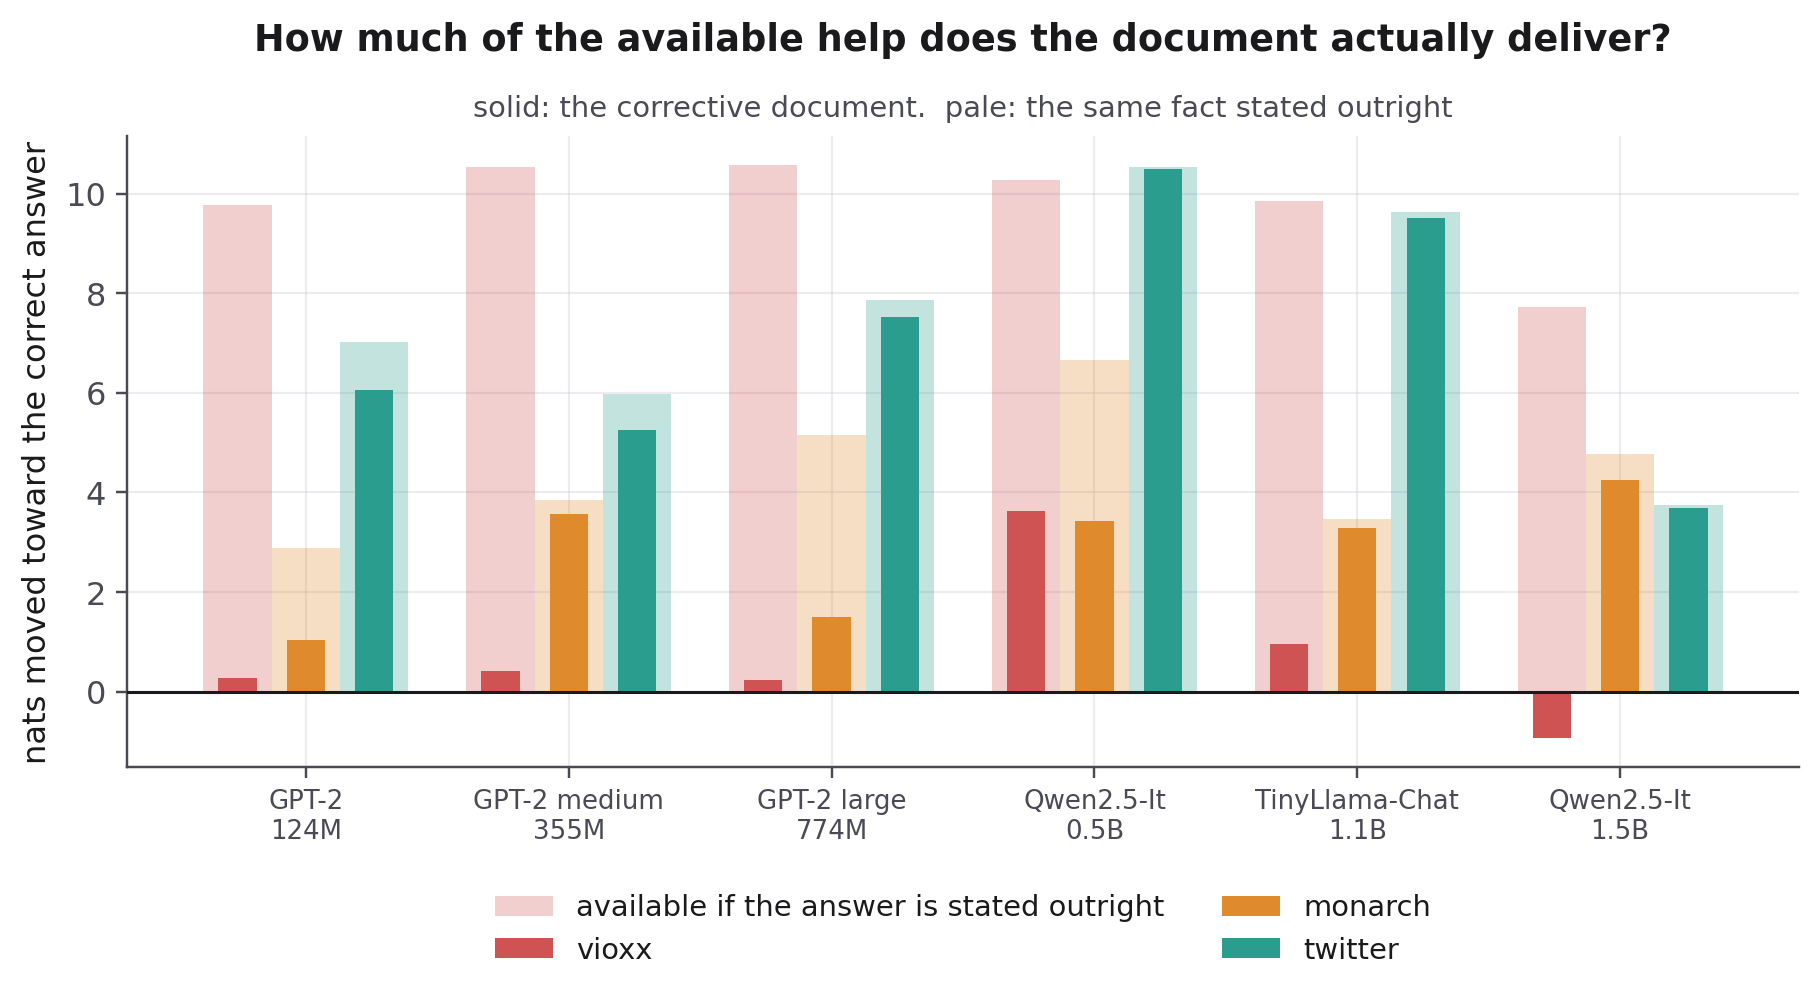
\includegraphics[width=0.86\linewidth]{figures/help.png}
\caption{How much of the available help the corrective document delivers. The
pale bar is the surprisal reduction available when the answer is stated outright;
the solid bar is what the corrective document achieves. On the Twitter probe the
document delivers nearly all of what is available. On Vioxx it delivers almost
none of roughly ten nats, and for the largest model it moves the correct answer
the wrong way.}
\label{fig:help}
\end{figure}

\paragraph{Two qualifications.} Qwen2.5-1.5B-Instruct answers ``
unsafe'' on the Vioxx probe. That is the right direction and the wrong token,
and the point-mass estimator scores it as a failure because it is defined
against one verified continuation; the estimator measures lexical recovery of a
specific answer, not semantic correctness, and this is the clearest case in the
data where the two come apart. Separately, the GPT-2 rows remain the
cleanest scale comparison, because family, tokenizer and training data are held
fixed there and only size changes.

% ============================================================
\section{Open Problems and Future Directions}
\label{sec:open_problems}
% ============================================================

\subsection{Unified Benchmarks for the Full Lifecycle}

The field needs benchmarks that test \textit{sequences} of lifecycle operations, not individual stages. A lifecycle benchmark would work as follows: (1) the system ingests a corpus of facts, (2) it is tested on retrieval accuracy, (3) a subset of facts is updated, (4) the system is re-tested to verify that updates have propagated and that non-updated facts are unaffected, (5) a subset of facts is marked for deletion, and (6) the system is tested to verify that deleted facts are truly inaccessible, including through indirect queries. Each step is straightforward; the value is in chaining them together and measuring the cumulative error. $\mathcal{D}_{sync}$ probes of the kind constructed in \S\ref{sec:case_study} supply the per-step measurement.

\subsection{Scaling the Desynchronization Measurement}

The single-probe measurement in this paper should become a benchmark: a curated set of documented fact changes (drug withdrawals, leadership changes, API deprecations, boundary revisions) paired with corrective documents, evaluated across model families and scales. Two axes matter most: how $\widehat{\mathcal{D}}_{sync}$ varies with model scale and instruction tuning, and whether reasoning-mode inference~\citep{openai2024o1, guo2025deepseekr1} reduces it, as the test-time resolution hypothesis (\S\ref{sec:update}) predicts it should. We report that sweep in \S\ref{sec:crossmodel}: across six open models and three probes, the conflict resolves readily on one probe, not at all on another, and non-monotonically with scale on the third. Whether reasoning-mode inference reduces $\widehat{\mathcal{D}}_{sync}$ where scale does not remains open.

\subsection{End-to-End Differentiable Knowledge Systems}

Current RAG pipelines are modular but non-differentiable: the retriever and the generator are trained separately, and the boundary between them is a hard discrete selection of top-$k$ passages. Early work on joint training~\citep{guu2020realm, izacard2023atlas} showed that end-to-end optimization improves both retrieval and generation. Extending this idea across the full lifecycle, jointly optimizing acquisition, storage format, retrieval strategy, update mechanisms, and forgetting policies, remains open: it would require differentiable approximations of inherently discrete operations such as database insertion and deletion.

\subsection{Multi-Modal Knowledge Lifecycles}

This paper focuses on text, but each new modality brings its own lifecycle challenges. Visual generative systems encode domain knowledge in their learned representations just as language models do, and they inherit the same staleness: stylization and cross-domain synthesis models generate from priors fixed at training time~\citep{thakur2021whitebox, thakur2021aoda}, with no mechanism to revise them when the domain moves. Zero-shot vision-language pipelines compound the problem, because a pipeline assembled from frozen components is only as current as the least current of them~\citep{thakur2026accident}. A vision-language model whose textual weights encode a drug's approval while an image in context shows its withdrawal notice faces the same boundary conflict measured in \S\ref{sec:case_study}, with the further question of which modality wins when they disagree. Extending the $\mathcal{D}_{sync}$ protocol to controlled text-image conflict pairs on open VLMs is an experiment we have scoped and intend to report separately; the measurement requires token-probability access to the fused decoder, which open models such as LLaVA provide.

\subsection{Knowledge Lifecycles for Multi-Agent Systems}

When multiple LLM agents collaborate, knowledge management becomes a distributed systems problem. Agents must share knowledge without creating inconsistencies, coordinate updates so that one agent's edit does not conflict with another agent's cached copy, and manage access control so that sensitive knowledge is available to authorized agents and hidden from others. The lifecycle framework suggests that each agent maintains its own local lifecycle while participating in a collective lifecycle at the system level. Distributed systems research provides decades of experience with consistency, replication, and conflict resolution; applying it to multi-agent LLM systems is largely unexplored~\citep{wang2024agents}.

% ============================================================
\section{Limitations}
\label{sec:limitations}
% ============================================================

First, the Provenance Vector is an architectural proposal supported by an idealized analysis, not a trained system. Proposition~\ref{prop:consistency} holds under strong assumptions, stated explicitly in \S\ref{sec:analysis_proof}, and the auxiliary provenance loss may interact with the language modeling objective in ways only a full pre-training run can reveal. We present it as a principled architectural direction, not a validated method.

Second, the empirical measurement covers three probe scenarios across six models from 124M to 1.5B parameters (\S\ref{sec:crossmodel}). It establishes that the failure mode exists, is measurable, is separable into retrieval and resolution components, and does not disappear with scale on the Vioxx probe; it does not establish prevalence across domains, nor behavior at frontier scale, nor under reasoning-mode inference. The point-mass estimator additionally assumes a single verifiable correct continuation, which fits factual probes but not open-ended queries, and it is sensitive to how the query is worded: across three phrasings of each probe the Vioxx measurement has a median standard deviation of 5.14 nats, and the phrasing reported here is the hardest of the three for every model tested (\S\ref{sec:crossmodel}). The estimator measures the conflict together with how readily the query frame admits the answer string, and those two are not separated here.

Third, the coverage analysis (Table~\ref{tab:coverage}) maps twenty representative works chosen to span the five subfields. A full bibliometric analysis would strengthen the fragmentation claim, though the qualitative pattern is consistent with the dedicated surveys of each subfield.

Fourth, the cross-modal extension of the metric is scoped but not yet executed; no multimodal measurement is reported in this paper.

% ============================================================
\section{Ethics and Broader Impact}
\label{sec:ethics}
% ============================================================

The lifecycle failures described in this paper carry direct societal consequences. In medicine, a desynchronized model that confidently recommends a withdrawn drug, as measured in \S\ref{sec:case_study}, could cause patient harm. In law, a model that fails to unlearn privileged client data after a deletion request violates confidentiality obligations and data protection regulations. In finance, a model whose parametric weights encode a pre-crisis market regime while its RAG index reflects current conditions may produce inconsistent risk assessments.

The Provenance Vector and the $\mathcal{D}_{sync}$ metric are designed to mitigate these risks, but they introduce new ones. Provenance metadata, if exposed, could reveal proprietary training data sources. $\mathcal{D}_{sync}$ audits could be used to identify and exploit model weaknesses rather than to remediate them. We urge practitioners to treat lifecycle-aware tools as components of a broader responsible deployment framework that includes human oversight, domain-expert review, and regulatory compliance.

% ============================================================
\section{Conclusion}
\label{sec:conclusion}
% ============================================================

This paper structures the fragmented study of knowledge in large language models, showing that five separately developed subfields (retrieval-augmented generation, knowledge editing, continual learning, context engineering, and agent memory) operate as interconnected stages of a single Knowledge Lifecycle: Acquisition, Storage, Retrieval, Update, and Forgetting. Mapping twenty representative works onto these stages shows a median coverage of two stages, and the least-studied boundaries between stages are precisely where deployed systems fail.

We contributed two technical components for those boundaries. \textbf{Lifecycle Desynchronization} ($\mathcal{D}_{sync}$) makes the boundary failure measurable: in a reproducible probe of a documented drug withdrawal, GPT-2 assigns the correct continuation probability $5.9 \times 10^{-6}$ with the corrective document present in context, while the document shifts the model's distribution by only $0.033$ nats. The \textbf{Provenance Vector} ($p$) addresses the failure's root cause, the absence of temporal metadata in parametric storage, by attaching provenance to each FFN memory slot and gating stale activations at inference time, with an idealized consistency result delimiting exactly what accurate provenance buys.

As language models transition into autonomous systems, knowledge management can no longer rely on the assumption that weights, indices, and contexts agree. The Knowledge Lifecycle framework supplies the shared vocabulary, the metric makes disagreement measurable, and the Provenance Vector offers one architectural path to closing the loop.

\appendix
\section{Glossary of Key Terms}
\label{sec:glossary}

\begin{itemize}[leftmargin=*]
  \item \textbf{Knowledge Lifecycle:} The unified framework consisting of five stages: Acquisition, Storage, Retrieval, Update, and Forgetting.
  \item \textbf{Parametric Storage:} Factual information encoded directly into the neural weights of a model, typically via pre-training or fine-tuning.
  \item \textbf{Non-Parametric Storage:} Information stored in external, modular indices such as vector databases, knowledge graphs, or document stores.
  \item \textbf{Retrieval-Augmented Generation (RAG):} The architectural pattern of retrieving external documents and injecting them into the context window to ground model generation.
  \item \textbf{Knowledge Editing:} The process of surgically modifying specific factual associations within a model's parametric weights.
  \item \textbf{Continual Learning:} The ability of a model to acquire new domains of knowledge over time without catastrophic forgetting.
  \item \textbf{Agent Memory:} The system-level hierarchy used to store interaction logs and user-specific knowledge across sessions.
  \item \textbf{Representation Engineering (RepE):} Controlling model behavior by monitoring and steering internal activations rather than modifying static weights.
  \item \textbf{Provenance Vector ($p$):} Proposed metadata embedding attached to each FFN memory slot, encoding acquisition time and source reliability for use by the inference-time gate.
  \item \textbf{Lifecycle Desynchronization ($\mathcal{D}_{sync}$):} Proposed metric quantifying the divergence between a deployed system's output distribution and that of a synchronized system, estimated in practice as the surprisal of the verified correct answer.
  \item \textbf{Context Influence ($\mathcal{I}_{ctx}$):} Companion diagnostic measuring how far the retrieved context moves the model's output distribution; small values with large $\mathcal{D}_{sync}$ indicate inert context.
  \item \textbf{Test-Time Compute:} Extra computational resources spent at inference time, through search or extended reasoning, to improve answer quality and conflict resolution.
\end{itemize}

\bibliographystyle{apalike}
\bibliography{references}

\end{document}
